\documentclass{article}
\usepackage[margin=2.5cm]{geometry}

\usepackage{amsmath}
\usepackage{amssymb}
\usepackage{amsfonts}
\usepackage{amsthm}

\usepackage{multicol}

\usepackage[magyar]{babel}
\usepackage{t1enc}

\usepackage[autostyle]{csquotes}
\selectlanguage{hungarian}

\usepackage{tikz}
\usetikzlibrary{positioning}

\title{Beosztások igazságosságának vizsgálata}
\author{Rónai-Kovács Martin}
\date{2022}

\theoremstyle{definition}
\newtheorem{definition}{Definíció}[section]
\newtheorem{theorem}{Tétel}[section]
\newtheorem{allitas}{Állítás}[section]
\newtheorem*{kov}{Következmény}
\newtheorem*{megj}{Megjegyzés}
\newtheorem{lemma}[theorem]{Lemma}

\newcommand{\set}[1]{ \{ {#1} \} }
\newcommand{\subin}[1]{ {#1}_{\text{in}} }
\newcommand{\subout}[1]{ {#1}_{\text{out}} }
\newcommand{\vect}[1]{ \underline{#1} }
\newcommand{\norm}[1]{ \parallel {#1} \parallel }
\newcommand{\pl}{ \textbf{Példa:} }
\newcommand{\ent}[2]{ {#1}^{(#2)} }
\newcommand{\info}[1]{ \text{inf}( #1 ) }

\begin{document}

\maketitle

\begin{multicols}{2}


    \begin{abstract}
        Ebben az összefoglalóban a beosztásokra vonatkozó igazságosság fogalmát próbáljuk megfogalmazni, mint általános mérték. Az ezzel kapcsolatos legnagyobb probléma, hogy a legtöbb beosztás esetén egyéni algoritmusok készítenek beosztásokat, egyéni be- és kimenetekre. Megállapítunk általánosítási eljárásokat és fogalmakat, és ezeket használva definiáljuk a hasonlóságot bemenetek között és az igazságosságot, mint az ettől való eltérés mértékét. \footnote{Ezt előre fogalmaztam meg, nem ez lesz ideírva}
    \end{abstract}

\section{Bevezetés}
    A beosztási problémák megoldása, lévén egy NP-teljes probléma, nagy körültekintést, hatékonyságot, és igen gyakran problémára specifikált megoldási módszert igényel. Emiatt kényszerűen el kell fogadnunk egy-egy elkészült beosztásról, hogy annál jobbat nem fogunk találni, megfelel a pszeudo-tökéletes eredmény is. 
    
    Ezzel az esetek nagy részében ki is lehet egyezni, azonban fontos kérdés, hogy milyen szempontból nem felel meg az adott beosztási eredmény. Egyes beosztásokban tapasztalható, hogy a beosztó algoritmus olyan szabályokat és egyszerűsítéseket tanul meg a már létező mintákból, amit mi nem szeretnénk figyelembe venni, például nemet, rasszot, kort, párkapcsolati státuszt, márkát, vagy bármi hasonlót. Ezt szeretnénk észrevenni.
    
    A beosztási probléma sokrétűsége miatt azonban ennek minden problémára születhet egyéni meghatározása és kimutatási algoritmusa, pont ugyanúgy, ahogy a beosztási algoritmus is általában egy-egy problémára születik meg.
    
    Ezt szeretnénk mi áthidalni azzal, hogy megállapítunk egy általánosított eljárást, amivel az igazságosság (amiről fentebb esett szó) mértéke megállapítható egy tetszőleges beosztási problémára készült beosztásról.
    
    A módszer megalkotása során következő célokat határozzuk meg:
    \begin{enumerate}
        \item A módszer legyen problémafüggetlen, ideértve a problémához tartozó be- és kimenetek szemantikáját és formátumát.
        \item A módszer legyen algoritmusfüggetlen, tehát ne vegye figyelembe a kapott be- és kimenet közti logikai kapcsolatot.
        \item A módszer a lehető legkevesebb emberi beavatkozást igényelje. Ez lényegében azért lesz fontos szempont, mert feltételezzük az igazságosság objektív létét, illetve el szeretnénk kerülni, hogy a megválaszolatlan kérdéseket problémafüggő megoldásokkal helyettesítsük.
        \item A módszer eredménye (kimenete) legyen számszerű; hiszen így állapítható meg, hogy egyes beosztások igazságosabbak, mint mások.
    \end{enumerate}
    
    Amit mi keresünk, az egy $f( \set{ I_S, O_S }) = \varphi \in \mathbb{R}$ függvény, ahol $\set{I_S, O_S}$ egy tetszőleges beosztási probléma be- és kimenete. Ezen $f$ megalkotásakor kell a fenti szempontokat megvalósítanunk.

\section{Beosztások közti reláció}
    
    \begin{definition}[Beosztás]
        A beosztás egy tetszőleges beosztási probléma egy bemenete és az arra (egy tetszőleges beosztáskészítő által) adott kimenet.
        \begin{equation} S = \set{I_S, O_S},\end{equation} 
        \\ ahol $I_S$ az $S$ beosztás bemenete, míg $O_S$ az $S$ beosztás kimenete.

    \end{definition}
    
    Tegyük fel, hogy a beosztásainkat elkészítő folyamat egy $\sigma$ függvény, tehát $\sigma(I_S) = O_S$. Logikus lehet feltételezni azt, hogy eltérő bemenetekhez nem minden $\sigma$ esetén lehet ugyanazt a kimenetet rendelni.
    

    \begin{theorem}
        \begin{equation}
            \exists \sigma \ : \ 
            \sigma(I_S)
            \not= 
            \sigma(I_\Sigma)
        \end{equation}
    \end{theorem}
    
    Ennek jelentősége, hogy a beosztásokban az igazságosságot a kimenetek is szabják; ha egy kimenet eleve nem lehet elég megfelelő (mert olyan \enquote{szerencsétlen} bemenethez tartozik), akkor a hozzá tartozó igazságossági mérték sem az adott beosztásról ad nekünk információt: előfordulhat, hogy egy megadott bemenethez a lehető legoptimálisabb beosztás igazságossága is rosszabb, mint egy másik bemenethez tartozó legrosszabb beosztásé.
    
    \begin{definition}[Izomorfia]
        Két beosztás pontosan akkor izomorf, ha azonos bemenetük van.
        \begin{equation} S \cong \Sigma \Longleftrightarrow I_S = I_\Sigma \end{equation}
        \begin{megj}
            Két beosztás pontosan akkor izomorf, ha a beosztási algoritmus átalakításával elérhető, hogy a kimenetek azonosak legyenek.
        \end{megj}
    \end{definition}
    
    \begin{theorem}\label{thm:trihotomia}
        Két beosztás igazságossága között csakis akkor létezik reláció, ha a beosztások izomorfak.
        \begin{equation} \exists \ \theta \in \set{<, >, =}: f(S)\ \theta\ f(\Sigma) \Longleftrightarrow S \cong \Sigma \end{equation}
        Azaz a trihotómia nem teljesül bármely két beosztás igazságosságára.
    \end{theorem}
    
\section{Általánosítás}
    
    Határozzuk meg pontosabban a bemenetet. Egy beosztás általában entitások egymáshoz rendeléseként fogható fel, talajdonképpen az előre ismert tulajdonságokhoz állapítunk meg relációkat és az ezekhez tartozó egyéb tulajdonságokat tudjuk még kiszámolni.
    
    \pl CPU-magok és feladatok esetén az entitásaink a magok és a feladatok. A kimenetünk az, hogy melyik feladatot melyik mag végzi el, illetve hogy melyik maghoz hány feladat tartozik (ez utóbbi egy számított tulajdonság). Kiszámítható még, hogy melyik magnak mekkora az összterhelése, de itt már számíthatunk idővel vagy feladatszámmal is (Ez még problémákhoz vezet, lásd később).
    
    Azonban a bemenetek leírása egyszerű: minden entitásunkat egy vektorként kell értelmezzük, melynek elemei a paraméterértékek. Mivel többféle vektorra lehet szükség (mert egy CPU-magot nem ugyanúgy írunk le, mint egy feladatot), ezért a vektorok mérete eltérő.
    
    Először határozzuk meg a beosztási problémát. Minden problémában entitások (beosztandók) és követelmények szerepelnek. Így adódik a következő egyszerű leírás:
    
    \begin{definition}[Beosztási probléma]\label{def:problema}
        Egy beosztási probléma definíciója a példányok leírásainak halmaza és a követelmények halmaza:
        \begin{equation}
            D_S = \set{E_S, C_S},
        \end{equation}
        ahol $E_S$ a probléma entitásainak leírásait (entitásosztályok), $C_S$ pedig a probléma követelményeit tartalmazza.
        \begin{megj}
            $E_S$ és $C_S$ pontos formájával nem kell foglalkoznunk, mert nem használjuk őket (ezek a $\sigma$ függvény definiálásához kellenek); elég tudnunk, hogy $E_S$ az entitásosztályok egy {\it halmaza}.
        \end{megj}
        \begin{megj} \label{megj:param_func}
            Az entitások itt nem nyers adatként jelennek meg. Úgy kell őket elképzelnünk, mint egy paraméterszámítási {\it függvény} eredményét ($p(r) = \varepsilon$), ami a nyers adatokból releványs információkat nyer ki számunkra. Erre azért van szükség, mert például záróvizsgabeosztásnál mindegy, mely hallgatókat vizsgáztatja egy oktató, a kérdés az, hány hallgatót vizsgáztat egy oktató.
        \end{megj}
    \end{definition}
    
    \begin{definition}[Csoport]
        Azon entitások, melyek egy osztályba tartoznak, egy csoportot alkotnak. Egy $e \in E_S$ osztályhoz tartozó csoportot a következőképpen definiálunk:
        \begin{equation}
            G(e) = \bigcup_{\varepsilon \ :: \ e} \varepsilon
        \end{equation}
        Ahol az $\varepsilon \ :: \ e$ jelentése, hogy $\varepsilon$ az $e$ osztályleírásnak megfelel. 
    \end{definition}
    
    \begin{definition}[Homogenitás]
        Két entitás homogén egymással, ha azonos osztályhoz tartoznak.
        \begin{equation}
            \varepsilon_1 \sim \varepsilon_2 \Longleftrightarrow \varepsilon_1 :: e \wedge \varepsilon_2 :: e
        \end{equation}
    \end{definition}
    
    Az egyes entitások leírása bővül a beosztás ($\sigma$) hattatása után, ezért érdemes megkülönböztetni a bemeneti és kimeneti állapotokat.
    
    \begin{definition}[Be- és kimeneti állapotleírás]
        Egy $\varepsilon$ entitás bemeneti leírása $\subin{\varepsilon}$, kimeneti leírása $\subout{\varepsilon}$; hasonlóan a be- és kimeneti osztályleírás $\subin{e}$ és $\subout{e}$.
    \end{definition}
    
    Ezen definíciók ismeretében már meg tudjuk határozni a bemenetet.
    
    \begin{definition}[Bemenet]
        A bemenet egy $S$ beosztásra ($I_S$) megegyezik a csoportok halmazával.
        \begin{equation}
            I_S = \bigcup_{e \in E_S} G(\subin{e}),
        \end{equation}
        tehát $I_S$ azonos méretű vektorok halmazainak halmaza.
    \end{definition}
    
    Az egyes entitásosztályok külön bemenetként való kezeléséhez határozzuk meg a csoportonkénti bemenetet:
    
    \begin{definition}[Csoportonkénti bemenet]
        Az $e$ entitásosztályhoz tartozó csoportonkénti bemenet $I_{S, e}$ megegyezik $\subin{e}$ csoportjával.
        \begin{equation}
            I_{S, e} = G(\subin{e})
        \end{equation}
    \end{definition}
    
    Tehát meghatároztuk a beosztási problémánk bemenetének leírását. Tételezzük fel, hogy a kimenetet hasonlóan írhatjuk le, tehát a fenti definíciókban $I_S$ felcserélhető $O_S$-sel, amennyiben az $\subin{e}$-t is felcseréljük $\subout{e}$-tal, stb.
    
    \begin{theorem}[Normalizáció I.]\label{thm:norm1}
        Minden bemenetnek létezik normáltja, vagyis
        \begin{equation}
            \forall I_{S,e} : \exists \norm{I_{S,e}} 
        \end{equation}
        \begin{proof}
        Használjuk az alábbi lemmát:
            \begin{lemma}[Entitás-vektor azonosság]\label{lem:vektor}
                Minden entitás leírható valós vektorként, azaz 
                $\varepsilon = \vect{\varepsilon} \in \mathbb{R}^n$, 
                ahol $n$ az $\varepsilon$ entitás paramétereinek száma (ideértve a számított paramétereket is).
            \end{lemma}
            $\parallel I_{S,e}\parallel $ azonos a benne lévő entitások normáltjaival, hiszen azok egymástól függetlenek. Mivel ezek valós vektorok $\mathbb{R}^n$-ben (\ref{lem:vektor}), létezik normáltjuk, és így $I_{S,e}$-nek is létezik normáltja.
        \end{proof}
        \begin{megj}
            A tétel fontossága, hogy tetszőleges beosztási problémánál a bemenetet általánosítani tudjuk.
        \end{megj}
        \begin{kov}
            Csakis akkor tudunk általánosítani, ha a bemeneti vektorok normálhatók.
        \end{kov}
    \end{theorem}
    
\section{Paraméterek függése}

    Az eddigiek alapján szeretnénk elérni, hogy az igazságossági függvény ($f$) bemenetei általánosak legyenek, és ehhez meghatároztuk a befogadható formákat. A teljes általánosításhoz azonban el kell végeznünk a normalizációt is, hogy tényleg tetszőleges entitásokkal tudjunk dolgozni. 
    
    A probléma itt a normalizációval van, hiszen meg kell határoznunk, hogy hogyan lehetne tulajdonságvesztés nélkül, a paraméterek egymáshoz való relációjának megtartásával együtt módosítani az entitásokat.
    
    Mivel 
    \begin{equation}
        \norm{I_S}  = \bigcup_{e\ \in \ E_S} \norm{I_{S,e}} ,
    \end{equation}
    a teljes bemenetet tudjuk normálni, amennyiben az csoportokat egyesével tudjuk normálni. Ezt meg tudjuk tenni, mivel a csoport entitásai egymástól függetlenek (ahogy azt \az{(\ref{thm:norm1})} tétel bizonyításakor feltételeztük).
    
    Logikusnak tűnhet, hogy (mivel valós vektorokról van szó) ezeket egész egyszerűen euklideszi hosszúsággal leoszzuk:
    $$ \parallel\vect{v}\parallel = \frac{1}{|\vect{v}|} \vect{v} $$
    így kapva egy egység hosszú vektort tetszőleges $\mathbb{R}^n$ térben. Azonban ezzel elkövethetjük azt a hibát, hogy két relatíve távoli pont távolságát 0-ra csökkentjük.
    
    \pl $\vect u = (0, 1, 1)$; \ $\vect v = (1, 1, 1)$; \ $\vect w = (10, 10, 10)$
    vektorok esetén normálás során $\vect v$ és $\vect w$ távolsága $15.588$-ról $0$-ra csökken, míg $\vect v$ és $\vect u$ távolsága $1$-ről $0.605$-re csökken; tehát a $\vect v - \vect w$ és $\vect v - \vect u$ közti reláció megfordul, ha ezeket egyesével normáljuk (jelen példában feltételeztük, hogy két vektor távolsága megegyezik azok különbségével).
    
    A példában látható jelenséget szeretnénk elkerülni, így máshogyan kell a normalizációt definiálnunk.
    
    \begin{definition}[Normalizáció]\label{def:norm}
        Egy $\vect\varepsilon$ entitás normáltja $\nu(\vect\varepsilon)$ (vagy $\norm{\vect\varepsilon}$). A normálás az azonos paraméterek közti relációt megtartja, de a vektort véges térbe transzformálja.
        \begin{equation}
            \nu : \mathbb{R}^n \to [r_1; r_2]^n,
        \end{equation}
        ahol $r_1, r_2 \in \mathbb{R}$ és $r_1 < r_2$.
        
        \begin{megj}
            Az azonos paraméterek közti relációt meg kell tartanunk, hogy ne forduljon elő a fenti példában látott eset (reláció megfordulása). További előny, hogy a paraméter normáltja ez esetben függeni fog a többi entitás értékskálájától, de nem függ a többi paramétertől.
        \end{megj}
        
        \begin{megj}
            A továbbiakban $r_1 = 0$ és $r_2 = 1$ értékekkel használjuk a normalizáció fogalmát.
        \end{megj}
    \end{definition}
    
    Hogy \az (\ref{def:norm}) definíciónak megfeleljünk, feltehetjük, hogy a paramétereket egyenként normálhatjuk. Ennek azonban van egy feltétele, ami az alábbi tételben olvasható.
    
    \begin{theorem}[Normalizáció II.]
        Amennyiben az entitás paraméterei függetlenek, az entitás normáltja megegyezik az entitás paramétereinek normáltjával:
        \begin{equation}
            \forall i \neq j \ : \ 
            \vect\varepsilon_i \not \propto \vect\varepsilon_j 
            \ \Longrightarrow \
            \norm{\vect\varepsilon}_i = \norm{\vect\varepsilon_i}
        \end{equation}
    \end{theorem}
    
    \begin{theorem}[Visszaállíthatóság]
        $\nu$ reverzibilis, $\exists \ \nu^{-1}$.
        
        \begin{proof}
            Mivel $f$ csak adott bemenetre ad számszerű értéket (\ref{thm:trihotomia}), ismerjük a teljes lehetséges értékkészletet minden paraméterre. Ebben az esetben (tehát mindig) belátható, hogy 
            $$ \nu_i(\varepsilon) : [r_1; r_2] \to [0; 1], $$
            ahol $r_1 = \arg_\varepsilon\min(\varepsilon_i)$ és $r_2 = \arg_\varepsilon\max(\varepsilon_i)$.
            Tudjuk, hogy minden entitásra igaz, hogy azonos paramétereik között a relációs viszony megmarad (\ref{def:norm}), így $\nu_i^{-1}$ maga is megfelel a normalizáció fogalmának. Ekkor könnyen választhatunk egy olyan értékkészletet, amely az eredeti paraméter értelmezési tartománya. Ezzel megalkottuk $\nu$ inverzét. (És megállapítottuk, hogy $\nu$ bijektív).
        \end{proof}
        \begin{megj}
            Ezzel beláttuk, hogy normalizáció során nem történik információvesztés.
        \end{megj}
    \end{theorem}
    
\section{Normalizációs problémák}
    A normalizációval beláttuk, hogy tetszőleges beosztási probléma (mely leírható \az{(\ref{def:problema})} formában) általánosítható. 
    
    Ennek azonban feltétele volt, hogy az osztályok, az entitások, és azok paraméterei egymástól függetlenek legyenek. Ez főként a $p$ függvény (\ref{megj:param_func}) megalkotásában jelentős szempont.
    
    A másik aggály, ami felmerülhet, hogy (véges pontosságú eszközök miatt) egyes adatok irrelevánssá válhatnak a normalizáció során. Például lehetnek olyan paraméterek, melyeket nem lineárisan, hanem logaritmikusan kell normálni, mivel maguk a paraméterek exponenciálisak. Ez a probléma elkerülhető, ha a normalizációs ($\nu_i$) függvényeket minden paraméterre körültekintően választjuk meg. Ez talán még automatizálható is regressziókkal.
    
    Ha a normalizáció során elérjük, hogy a skálán elhelyezkedő értékek ugyanolyan eloszlásúak legyenek (lehetőleg lineárisak), akkor tetszőleges paraméter {\it tekinthető} lineárisnak. Ennek jelentősége a továbbiakban jelentős, hiszen ezzel elérjük, hogy két entitás távolságának számításakor a paraméterek homogének legyenek eloszlás szempontjából (tehát ne kelljen minden paraméterre meghatározni egy \enquote{távolságbefolyásolási tényezőt}, vagy hasonlót).
    
\section{Távolságok}    
    
    A távolságok nagy szerepet játszanak az igazságosság megállapításában, hiszen a beosztás előtti és utáni távolságok közti eltérésből deríthetjük ki a legszembetűnőbb anomáliákat (ha csak 1GHz-es CPU-ink vannak, rendben van, hogy mind ugyanannyi feladatot kap; de ha van mellette egy 10GHz-es is, akkor az egyenlő szétosztás nem igazságos).
    
    Mivel a bemeneteken azok a paraméterek, melyeket csak a beosztás befolyásol nem lesznek egymástól távoliak (mindegyik alapértéken lesz), feltehető, hogy a bemeneteken a távolságok kisebbek, mint a kimeneten:
    $$ d_{in}(x, y) \leq d_{out}(x, y) $$
    
    Ugyanezt megfogalmazhatjuk egyszerűbben, ha a be és kimeneten ugyanaz a függvény méri a távolságot ($d_{in} \Leftrightarrow d_{out}$):
    \begin{equation}
        d(\subin{x}, \subin{y}) \leq d(\subout{x}, \subout{y})
    \end{equation}
    
    Itt egy feladatunk maradt: határozzuk meg $d$-t.
    
    \begin{definition}[Távolságfüggvény]
        Az igazságossági távolságfüggvény két azonosan paraméterezett entitásról ad olyan arányszámot, melyből azoknak különbözősége megállapítható. A beosztásban akkor állapíthatunk meg igazságtalanságot vagy igazságossági anomáliát, ha a be- és kimeneten mért távolságok jelentősen eltérnek.
        \begin{equation}
            d: \mathbb{R}^{2|e|} \to \mathbb{R}
        \end{equation}
        ahol $|e|$ az $e$ entitásosztály paramétereinek száma (azaz egy $\varepsilon :: e$ vektor mérete).
    \end{definition}
    
    Amennyiben valóban feltehetjük, hogy a paraméterek eloszlása azonos, minden két példány paraméterein ugyanazt a műveletet kell elvégeznünk, majd egyetlen összegző művelettel megállapíthatjuk, hogy az ezen paramétereket tartalmazó entitások távolsága mekkora. 
    
    \begin{definition} (Távolság) \label{def:tavolsag}
        Két entitás távolsága az őket leíró vektorok euklideszi távolsága (lineáris eloszlású normáltak esetén \footnote{Szükség van linearitásra? Nem elég, ha mind ugyanolyan? Egyáltalán ez az engedmény valóban engedmény lenne (azon kívül, hogy általánosabb esetet fedne a definíció)?}).
        \begin{equation}
            d(x, y) = \sqrt{\sum_{i=1}^{|e|} (x_i - y_i)^2 } 
        \end{equation}
        ahol $x \sim y$.
    \end{definition}
    
    Ezután állapítsuk meg, miért fontos ez számunkra. Igazságosnak akkor tekintünk egy beosztást, ha a beosztás elkészítése során nem torzítjuk azokat a távolságokat, melyek már a bemeneten is léteznek. Ezt felfoghatjuk úgy is, mint a Lipschitz-tulajdonság betartását (valamely $M$ konstansra):
    \begin{equation}
        \forall x \sim y : \ d(\subin{x}, \subin{y}) \leq Md(\subout{x}, \subout{y})
    \end{equation}
    
    Egy beosztástól azt szeretnénk, hogy a kimenetek távolságai arányosságban álljanak a bemeneti távolságokkal, tehát legyen igaz, hogy
    \begin{equation}
        d(\subout x, \subout y) \propto d(\subin x, \subin y).
    \end{equation}
    
    \begin{definition}[különbségváltozás, $\delta$]
        Két egymással homogén entitás különbségváltozása megegyezik a bemeneti és kimeneti különbségük közti eltéréssel. Jele: $\delta$.
        \begin{equation}
            \delta(x, y) = |d(\subout x, \subout y) - d(\subin x, \subin y)|
        \end{equation}
    \end{definition}

    Az eddigiekből következik, hogy a fairness-függvény értéke az egyes párok $\delta$-jából lesz számítva; ezt az átszámítást végezze esetünkben egy $u$ (unfairness) függvény, $f_e$ jelezze az $e$ entitásosztályon belüli igazságosságot:
    \begin{equation}
        f_e(S) \propto u_e\left(\ \bigcup_{x \sim y} \delta(x, y)\ \right)
    \end{equation}
    ahol $x::e$. Ezután a teljes fairségről megállapíthatjuk az egyszerű összefüggést:
    \begin{equation}
        f(S) \propto \sum_{e \in E_S} f_e(S)
    \end{equation}
    
    Az eddig megállapítottakat kell a fairness-függvény megalkotásakor figyelembe vennünk; ez alól kivétel a $d$ pontos definíciója, hiszen az euklideszi távolság valódi távolságot mér két entitás között \footnote{Ha egy paraméter pl. $e^x$ jellegű értékeket vesz fel, azaz exponenciális eloszlású, akkor a paraméteren mért távolság torz; ezért figyelnünk kell a normáltakra, hogy lineárisak legyenek.}.
    

\section{Súlyozás}
    Felmerülhetnek az igazságossággal kapcsolatban további kérdések, melyek megválaszolásával optimálisabb vagy akár gyorsabban számítható eredményeket kaphatunk. Ilyen lehet például, hogy minden entitás közti igazságosság kell-e (pl. időszeletek egyformasága számít?), vagy vannak-e olyan paraméterek, amiket érzékenyebben kell kezelnünk, mint a többit (pl. a \enquote{rassz} vagy \enquote{párkapcsolati státusz} tulajdonság és a hitelbírálat sikeressége nem jó, ha korrelál, így ezt érzékenyebben vizsgálhatjuk $f$-hez).
    
    Paraméterek fontosságának kijelentéséhez definiáljuk a súlyokat.
    
    Innentől jelölje jobb felső indexben zárójelezett változó az entitás osztályát: $x^{(e)} \Leftrightarrow x::e$.
    
    \begin{definition}[Súly]
        Egy osztály egy példányának $\ent{x}{e}_i$ paraméteréhez tartozó súlya azt fejezi ki, mennyire befolyásolja a fairséget egy $y\sim x$ példány $\ent{y}{e}_i$ paraméterétől való eltérés. 
        
        Ezen súly minden esetben nem negatív értéket vesz fel.
        \begin{equation}
            \ent{\vect w}{e} \in [0;\infty)^{|e|}
        \end{equation}
    \end{definition}
    
    \begin{definition}[Súlyozott entitás]
        Egy entitás súlyozása a paraméterenkénti szorzat számításából adódik:
        \begin{equation}
            \ent X e = \ent w e \ent x e
        \end{equation}
    \end{definition}
    
    \begin{definition}[Súlyozott (rész)távolság]
        A súlyozott távolság megegyezik a paraméterenkénti távolságok súlyokkal vett szorzatából számított távolságokkal. Az $i.$ résztávolság jele $d_i$:
        \begin{equation}
            d_i(x, y) = d(x_i, y_i),
        \end{equation}
        a súlyozott résztávolságok ekkor:
        \begin{equation}
            D_{i}(x, y) = w_id_i(x, y)
        \end{equation}
        \begin{megj}
            Mi esetünkben $d(x, y) = |x-y|$, tehát
            \begin{equation}\label{eq:sulyozott_euklideszi}
                D(x, y) = \sqrt{\sum_{i=1}^{|e|} D_i^2(x, y)} 
            \end{equation}
        \end{megj}
    \end{definition}
    
    \begin{megj}
        Ha $\ent w e$ minden eleme $1$, akkor a súlyozás eredeti állapotot hagy, míg ha minden eleme $0$, akkor az összes létező beosztást \enquote{igazságosra} módosítja.
    \end{megj}
    
    \begin{allitas}
        Amennyiben $d$ az euklideszi távolság, azaz $d(x,y) = |\vect x - \vect y|,$ akkor a különbségenkénti súlyozás helyettesíthető entitássúlyozással.
        \begin{proof}
            Határozzuk meg $d_i(x, y)$-t:
            \begin{equation}
                d_i(x,y) = |\vect x_i - \vect y_i|,
            \end{equation}
            tehát
            \begin{equation}
            \begin{split}
                D_i(x, y) &= w_i d_i(x, y) \\
                &= w_i |x_i - y_i| \\
                &= |w_i x_i - w_i y_i| \\
                &= d_i(wx, wy)
            \end{split}
            \end{equation}
            (\ref{eq:sulyozott_euklideszi}) ismeretében belátható, hogy euklideszi távolságok esetén a súlyozott résztávoságokból számított $d$ valóban megegyezik a súlyozott entitásokból számított $d$ értékével.
        \end{proof}
        \begin{megj}
            Ennek hasznossága leginkább, hogy $D(x, y)$ számításakor nem kell elvégeznünk a $w_i$-vel való szorzásokat minden $(x,y)$ párra, elég a számítás előtt minden $\varepsilon$ entitást felskálázni $w$-vel.
        \end{megj}
    \end{allitas}
    
    \begin{theorem}[Awareness - unawareness átjárhatóság]
        Bináris súlyok használatával elérhető, hogy a \textit{fairness through unawareness} (FTU) definíciót felhasználjuk, annak ellenére, hogy a \textit{fairness through awareness} (FTA) szerint haladt az eddigi gondolatmenetünk. 
        
        Ekkor az érdektelen változók súlyát 0-ra, a többi súlyt 1-re kell beállítanunk, így kapva egy $f_1$ fairness értéket; majd minden súlyt 1-re állítva kapunk egy $f_2$ értéket. Ezek különbsége mondja meg, hogy az FTU definíció szerint igazságos-e az adott beosztás:
        $$ |f_1 - f_2| < h_{FTU} \Leftrightarrow S \text{ igazságos}, $$
        ahol $h_{FTU}$ egy hibahatár.
    \end{theorem}
    
    Alapvetően a súlyozás optimalizásra használható, azonban lehetőséget ad arra is, hogy bizonyos információkat \enquote{enyhítsünk}, ha azok esetleg redundánsak lennének. Eddig ezt azzal a feltevéssel hidaltuk át, hogy az entitásainkat és azok paramétereit is páronként függetlennek tekinthettük, de így korlátoztuk $I_S$ formátumát, ezzel szűkítve a lehetséges $\sigma$ függvények, illetve a lehetséges $D_S$ leírások halmazát.
    
    Ennek áthidalása tehát kényelmes lenne, ezért vizsgáljuk meg, hogyan segíthetnek a súlyozások.

    Paraméterek esetén, ha több is ugyanazt az információt hordozza magában, tehát valamely $e$-re $$\forall x::e : \ \ent x e _i \propto \ent x e _j,$$ vagy máshogyan kifejezve $e_i \propto e_j$, akkor (hiába lehetséges, hogy eltérően definiálja $p$ ezen értékeket) az információt redukálnunk kell 1 paraméterbe.

    \begin{theorem}
        Súlyokkal elérhető, hogy a redundáns paraméterek információja ne legyen túlreprezentálva.
        
        \begin{proof}
            T.f.h. valamely $R \subset \ent x e$ egy olyan paraméterhalmaz, melynek minden eleme ugyanazt az információt hordozza, azaz teljesen redundáns paraméterek. (Ez nem azonos azzal, hogy két paraméter \textit{értéke} megegyezik!)
            
            Ekkor normálás után $\forall i: R_i \in [0;1]$, tehát súlyuk a távolságszámításban azonos (figyelembe nem véve a $\ent w e$ együtthatókat). 
            
            Amit el szeretnénk érni, hogy az $R$-beli értékek összesen akkora súlyúak legyenek, mint egyetlen paraméter. Ezt (az azonos értékkészlet miatt) megtehetjük úgy, hogy $\frac{1}{|R|}$ együtthatót adunk nekik.
            
            Alapvetően ezt akkor tehetjük meg, ha teljes a redundancia; de ezt feltételezhetjük, mivel minden egyes paraméter (a problémánk szempontjából) elemi információ (tehát nincs részleges függés).
        \end{proof}
    \end{theorem}
    
    \begin{definition}[Redundanciaegyüttható]
        Amennyiben két (vagy több) paraméter egy $e$ osztályban redundáns, redundanciaegyütthatójuk egy olyan érték, mellyel elérjük, hogy összesen akkora értékűek legyenek, mint egyetlen független paraméter.
        
        $R(\ent x e _i)$ azon paraméterek halmaza, melyek redundánsak $\ent x e _i$-vel.
        \begin{equation}
            \forall \ent x e _i \propto \ent x e _j : \ent x e _j \in R(\ent x e _i) 
        \end{equation}
        Ezt használva könnyen definiálható a redundanciaegyüttható:
        \begin{equation}
            \ent r e _i = \frac{1}{|R(\ent x e _i)|}
        \end{equation}
    \end{definition}
    
    \begin{definition}[összesített együttható, korrigált távolság]
        Egy $e_i$ paraméter összesített együtthatója $\ent c e _i$ megegyezik $e_i$ összes együtthatójának szorzatával. Mi esetünkben ez:
        \begin{equation}
            \ent c e _i = \ent r e _i \ent w e _i
        \end{equation}
        Ezzel újradefiniálható a korrigált (rész)távolság is:
        \begin{equation}
            D_i(x, y) = c_i d_i(x, y)
        \end{equation}
    \end{definition}

\section{Súlyozási problémák}
    Láttuk, hogyan alkalmazható a súlyozás a fairség hatékonyabb megállapításához, de természetesnek vettük, hogy a súlyok előre meg vannak állapítva. Azonban a kijelölt célok közül az elsőt (eddigi tudásunk szerint) megszegi minden olyan eset, ahol létezik $\ent w e _i \neq 1$, mivel ez esetben kézzel kell beállítani $w$ értékét (hiszen ez a paraméter \enquote{fontosságát} fejezi ki, tehát problémától és szemantikától nem független).
    
    Megoldás lehet, ha találunk algoritmust ezen súlyok automatikus megállapítására, de ekkor elveszhet $w$ eredeti célja. Itt inkább köztes megoldásra lesz szükség.\footnote{Köztes megoldás lehet, ha véletlenszerűen inicializált értékekkel töltjük fel a vektorokat, kiszámoljuk az így kapott $f$-et, optimalizáljuk az értékeket egy $\pm \gamma$-val való növeléssel, és ezt addig ismételjük, míg $f$ értéke maximális lesz. A folyamat leállásakor megtekintjük a kiszámolt $w$ értékeit, és megállapítjuk, reálisak-e.}
    
    $\ent r e$ meghatározása is hasonló problémákat vet fel, azonban a redundancia megállapítására léteznek módszerek, ez nem (feltétlenül) igényel emberi beavatkozást.
    
    További probléma a redundanciaegyütthatókkal, hogy a fentebb leírtak szerint csak akkor használhatóak, ha a paraméterek elemi információt hordoznak; ami egy újabb követelményünk $p$ megalkotásához.
    
    Végül feltehetjük a kérdést, hogy ha részben meg szerettük volna oldani a függetlenség kérdését, akkor miért nem oldottuk meg teljesen? Jelenleg nincs módszerünk arra, hogy a nem elemi információk közti redundanciát kezeljük. Entitások között fennállhat együttmozgás, ha a reprezentációs modell úgy határozza meg a problémát.
    
    \pl Zárovizsgabeosztás esetén szerepelhet a modellben \textit{Vizsgáztató}, de nem szerepelhet \textit{Elnök} és \textit{Belső tag}, mert megeshet, hogy ezeket a szerepeket ugyanaz az ember tölti be, így (az utóbbi modellben) effektíve kétszer reprezentálunk egy példányt.

\section{Igazságosság megállapításának folyamata}
    ...
    
    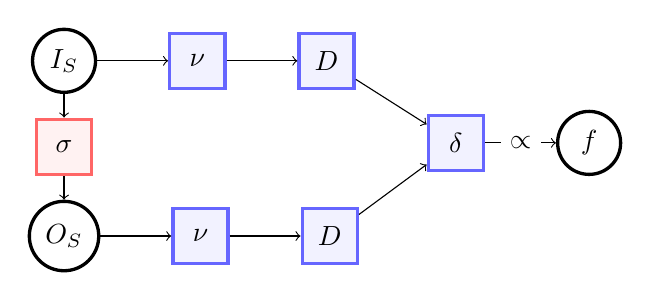
\begin{tikzpicture}[
        inoutput/.style={circle, draw=black, very thick, minimum size=8mm},
        red/.style={rectangle, draw=red!60, fill=red!5, very thick, minimum size=7mm},
        blue/.style={rectangle, draw=blue!60, fill=blue!5, very thick, minimum size=7mm},
        node distance= 3mm and 9mm
        ]
        
        \node[red]      (sigma)                                 {$\sigma$};
        \node[inoutput] (IS)                [above=of sigma]    {$I_S$};
        \node[inoutput] (OS)                [below=of sigma]    {$O_S$};
        
        \node[blue]      (normIn)           [right=of IS]       {$\nu$};
        \node[blue]      (normOut)          [right=of OS]       {$\nu$};
                
        \node[blue]      (dIn)              [right=of normIn]   {$D$};
        \node[blue]      (dOut)             [right=of normOut]  {$D$};
        
        \node[blue]      (delta)            [below right=of dIn]{$\delta$};
        
        \node[inoutput]  (fairness)         [right=of delta]    {$f$};
        
        %Lines
        \draw[->] (IS) -- (sigma);
        \draw[->] (sigma) -- (OS);
        \draw[->] (IS) -- (normIn);
        \draw[->] (OS) -- (normOut);
        \draw[->] (normIn) -- (dIn);
        \draw[->] (normOut) -- (dOut);
        \draw[->] (dIn) -- (delta);
        \draw[->] (dOut) -- (delta);
        \draw[->] (delta) -- (fairness) node[pos=0.5,fill=white] {$\propto$};
            
    \end{tikzpicture}

\section{Algoritmusfüggetlenség}
    ...
    
\end{multicols}
    
\end{document}
